% Preheader
%%%%%%%%%%%%%%%%%%%%%%%%%%%%
%%% DOCUMENT
%%%%%%%%%%%%%%%%%%%%%%%%%%%%

\documentclass[12pt,a4paper,captions=tableheading]{article}
% you may add/remove "twoside" above
% or "12pt"



%%%%%%%%%%%%%%%%%%%%%%%%%%%%
%%% TIMES-LIKE FONT
%%%%%%%%%%%%%%%%%%%%%%%%%%%%
\usepackage{mathptmx}



%%%%%%%%%%%%%%%%%%%%%%%%%%%%
%%% FONTS ETC.
%%%%%%%%%%%%%%%%%%%%%%%%%%%%

\usepackage[skip=15pt]{caption}
\usepackage[utf8]{inputenc}
\usepackage[T1]{fontenc}
\usepackage[english]{babel}
\usepackage{amsmath}
\usepackage{amsfonts}
\usepackage{amssymb}

%%%%%%%%%%%%%%%%%%%%%%%%%%%%
%%% CODE HIGHLIGHTING
%%%%%%%%%%%%%%%%%%%%%%%%%%%%
\usepackage{fancyvrb}  
\usepackage{minted} 
\usepackage{helvet}

\usepackage{xcolor}
\definecolor{border}{HTML}{ff5500}

\usepackage{tcolorbox}
\usepackage{etoolbox}
% for angular corners, Argument: arc is angular
\BeforeBeginEnvironment{minted}{\begin{tcolorbox}[colback=white, colframe=border, boxrule=0.4mm, arc=15px]}
\AfterEndEnvironment{minted}{\end{tcolorbox}}

%\setminted{style=abap}
\setminted{style=arduino}
\usepackage{fancyhdr}
%%%%%%%%%%%%%%%%%%%%%%%%%%%
%%% MISC USEPACKAGES
%%%%%%%%%%%%%%%%%%%%%%%%%%%% 
% font to Times
%\fontfamily{ptm}\selectfont
% font Arial

%\renewcommand{\familydefault}{\sfdefault}
% for figures
\counterwithin{figure}{section}
\usepackage{graphicx}
\graphicspath{ {./graphics/} }
% for the Distances
\usepackage[left=1.50cm, right=1.50cm, top=3.00cm, bottom=2.00cm]{geometry}
% für comment section
\usepackage{verbatim}
% für Zeilenabstand 1,5
\usepackage[onehalfspacing]{setspace}
% for spacing \hlines, default was 3pt,
% but led to a weird overall layout
\usepackage{tabularx}
% for long tables
\usepackage{longtable}
% to use the title and author
%\usepackage{titling}
% the options avoid boxes around the links
\usepackage[colorlinks=false, pdfborder={0 0 0}]{hyperref}
% for bibliography
\usepackage[numbers,square,sort]{natbib}
\bibliographystyle{unsrt}
% for subfigures
\usepackage[caption = false]{subfig}
%\usepackage{subcaption}
%for graphic/ table positioning
\usepackage{float}
%Hurenkind und Schusterjunge unterbinden
\usepackage[subfigure]{tocloft}
\clubpenalty=10000
\widowpenalty=10000
%for no shifting at the beginning of paragraph
\parindent 0pt
%for section in equation number
\numberwithin{equation}{section}
% rotating tables
\usepackage{rotating}
% degree
\usepackage{textcomp}
%line overflow handling
\setlength{\emergencystretch}{10em}
% multirow tables
\usepackage{multirow}
% si units
\usepackage[per-mode = fraction, exponent-product = \cdot, locale = DE]{siunitx}
% variable space
\usepackage{xspace}
%for graphic/ table positioning
\usepackage{float}
%für das Einbinden von Tabellen
\usepackage{booktabs}
%quotation
\usepackage{csquotes}
%abkürzungsverzeichnis
\usepackage[printonlyused]{acronym}
\usepackage{booktabs}
\usepackage{enumitem}

\renewcommand{\labelenumii}{\arabic{enumi}.\arabic{enumii}}

%%%%%%%%%%%%%%%%%%%%%%%%%%%%
%%% FORMAT
%%%%%%%%%%%%%%%%%%%%%%%%%%%%

\renewcommand{\cftfigpresnum}{Figure }
\renewcommand{\cfttabpresnum}{Table }
\renewcommand{\listoflistingscaption}{Sourcecode}
\renewcommand{\listingscaption}{Sourcecode}
\renewcommand{\cftfigaftersnum}{:}
\renewcommand{\cfttabaftersnum}{:}

\setlength{\cftfignumwidth}{2.7cm}
\setlength{\cfttabnumwidth}{2.7cm}
\linespread{1.25}
\setlength{\cftfigindent}{0cm}
\setlength{\cfttabindent}{0cm}
% Document

\begin{document}
	
	% Add title without page numbering or any other format
	\pagenumbering{Roman}
	\pagestyle{empty}
	%% Deckblatt
%\thispagestyle{TitelSeite}
\thispagestyle{empty}
\begin{verbatim}


\end{verbatim}

\begin{center}
\large{\textbf{ Development Notes }}

\end{center}

\begin{verbatim}


\end{verbatim}

\begin{center}
	\makebox[\linewidth]{\rule{\linewidth}{0.4pt}}
\end{center}


\begin{center}
	
	\textbf{\LARGE Design and development of an embedded system for controlling RGB LED fixtures}
\end{center}

\begin{center}
	 \large Controlling RGB LED fixtures with dedicated hard- and software subsystems in an combined embedded system
	  \makebox[\linewidth]{\rule{\linewidth}{0.4pt}}
\end{center}

\begin{verbatim}
	
	
\end{verbatim}

\begin{center}
	by Niko Kassubek
\end{center}
%% Ende des Deckblatts

	% Display page numbering
	\pagestyle{plain}

	% Table of contents
	\phantomsection
	\addcontentsline{toc}{section}{Contents}
	\tableofcontents
	\newpage
	
	\renewcommand{\arraystretch}{1.5}
	
	% abbreviations
	%%%%%%%%%%%%%%%%%%%%%%%%%%%%%%%%%%%%%%%%%%
%%%%%%%% INDEX OF ABBREVITATIONS %%%%%%%%%
%%%%%%%%%%%%%%%%%%%%%%%%%%%%%%%%%%%%%%%%%%
\phantomsection
\addcontentsline{toc}{section}{List of Abbreviations}

\section*{List of Abbreviations}
\begin{acronym}[1234567890]\itemsep1pt
	\acro{3D}[3D]{Three-Dimensional}
	\acro{CAD}[CAD]{Computer-Aided Design}
	\acro{COB}[COB]{Chip-on-Board}
	\acro{DC}[DC]{Direct Current}
	\acro{DCDC}[DC-DC]{Direct Current to Direct Current}
	\acro{DMX}[DMX]{Digital Multiplexing}
	\acro{EDA}[EDA]{Electronic Design Automation}
	\acro{EEPROM}[EEPROM]{Electrically Erasable Programmable Read-Only Memory}
	\acro{HMI}[HMI]{Human-Machine Interface}
	\acro{HSV}[HSV]{Hue, Saturation, Value}
	\acro{I2C}[I2C]{Inter-Integrated Circuit}
	\acro{IC}[IC]{Integrated Circuit}
	\acro{IO}[I/O]{Input/Output}
	\acro{IP}[IP]{Internet Protocol}
	\acro{IPA}[IPA]{Isopropyl Alcohol}
	\acro{LED}[LED]{Light-Emitting Diode}
	\acro{MCU}[MCU]{Microcontroller Unit}
	\acro{MOSFET}[MOSFET]{Metal-Oxide-Semiconductor Field-Effect Transistor}
	\acro{OLED}[OLED]{Organic Light-Emitting Diode}
	\acro{PCB}[PCB]{Printed Circuit Board}
	\acro{PWM}[PWM]{Pulse Width Modulation}
	\acro{RGB}[RGB]{Red Green Blue}
	\acro{RJ45}[RJ45]{Registered Jack 45}
	\acro{RS485}[RS485]{Recommended Standard 485}
	\acro{SMD}[SMD]{Surface-Mount Device}
	\acro{THT}[THT]{Through-Hole Technology}
	\acro{USB}[USB]{Universal Serial Bus}
	\acro{WLAN}[WLAN]{Wireless Local Area Network}
\end{acronym}


	\newpage
	
	\renewcommand{\arraystretch}{1.25}
	% list of figures
	\phantomsection
	\addcontentsline{toc}{section}{\listfigurename}
	\listoffigures
	\newpage

	% list of tables
	\phantomsection
	\addcontentsline{toc}{section}{\listtablename}
	\listoftables
	
	\newpage
	
	% list of Programmcode
	\phantomsection
	\addcontentsline{toc}{section}{Source Code}
%	\lstlistoflistings	
	\listoflistings
	\newpage
	
	% Include the abstract
	%\phantomsection
	%\input{./chapter/abstract}
	%\newpage
	
	% nomenklatur
	%\input{./chapter/nomenklatur}
	%\newpage

	% change page and chaper numbering
	\pagenumbering{arabic}
	\setcounter{section}{0}


	%%%%%%%%%%%%%%%%%%%%%%%%%%%%%%%%%%%%%%%%%%%%%%%
	%%%%%%%%%%  MAIN PART
	%%%%%%%%%%%%%%%%%%%%%%%%%%%%%%%%%%%%%%%%%%%%%%%
	\pagestyle{fancy}
	\fancyhf{} % Clear all header and footer fields
	\fancyhead[C]{\nouppercase{\leftmark}} % Place the current section title on the left side of the header
	\fancyfoot[C]{\thepage} % Place the page number on the right side of the footer
	\renewcommand{\headrulewidth}{0pt} % Optional: Remove the line above the header
	\renewcommand{\footrulewidth}{0pt} % Optional: Remove the line above the footer
	% ADD YOUR CHAPTER HERE
	\section{Introduction}
\label{sec:introduction}
\subsection{Motivation}
\subsection{Problem Statement and Objectives}
\subsection{Structure of the Article}
\textit{(These subsections remain largely the same)}
	\newpage
	\section{Theoretical Background}
\label{sec:theoretical_background}
\subsection{Embedded Systems}
An embedded system is fundamentally a computer system designed for a specific, dedicated function within a larger mechanical or electrical system. It comprises a combination of hardware, typically centered around a processor or \ac{MCU}, memory for storing software and data, and peripheral \ac{IO} devices for interacting with the external environment or the larger system it controls. Unlike general-purpose computers, embedded systems are often constrained by factors such as cost, size, power consumption, and real-time performance requirements, and their software, known as firmware, is specifically tailored to their dedicated task. The \ac{LED} controller developed in this work is an example of such an embedded system.

\subsection{RGB LEDs and Control Methods}
\ac{RGB} \ac{LED}s are semiconductor light sources that combine three individual \ac{LED} elements: red, green, and blue within a single package. By varying the intensity of each primary color, a wide spectrum of colors, including white, can be produced through additive color mixing. Controlling these \ac{LED}s typically involves one of two primary methods relevant to this project. The first method uses \ac{PWM} signals applied independently to each color channel of non-addressable \ac{LED}s, allowing for intensity control of the entire strip or fixture as a single unit. The second method employs addressable \ac{LED}s, where each \ac{LED} (or a small group) incorporates an \ac{IC}. These \ac{IC}s allow the \ac{LED}s to be connected in series and controlled individually via a serial data protocol, enabling complex effects and patterns across the length of an \ac{LED} strip or within a fixture. The choice of control method depends on the specific application requirements, balancing factors like cost, complexity, and the desired level of control granularity.

\subsection{Communication Protocols}
The embedded \ac{LED} controller supports industry-standard communication protocols for receiving lighting control data, enabling integration into various professional and hobbyist setups. Wired communication is primarily handled via the \ac{DMX} protocol, technically known as DMX512. \ac{DMX} is a unidirectional, serial digital protocol transmitted over an \ac{RS485} physical layer, designed for controlling stage lighting and effects. It allows for the addressing and control of up to 512 individual channels within a single "universe," typically corresponding to parameters like intensity or color values for different fixtures. The controller implements \ac{DMX} reception capabilities, allowing it to act as a DMX-controllable device.\\

For network-based control, particularly over wireless networks, the controller utilizes the Art-Net protocol. Art-Net is designed to transmit \ac{DMX} data packets over \ac{IP} networks, leveraging standard networking infrastructure like Ethernet or \ac{WLAN}. This allows for significantly larger systems spanning multiple \ac{DMX} universes and facilitates control from software or consoles connected to the same network. The controller's integrated \ac{WLAN} interface enables it to receive Art-Net commands wirelessly, translating them into the appropriate \ac{LED} output signals. The support for both \ac{DMX} and Art-Net provides flexibility in how the controller is integrated and controlled within a lighting system.

\subsection{User Interface Components}
The primary components facilitating user interaction with the embedded \ac{LED} controller constitute the device's \ac{HMI}. These components allow the user to configure settings, select operating modes, and view status information directly on the device.\\

The main input mechanism is a rotary encoder combined with an integrated push button. This single component serves multiple roles: rotation is used for navigating through menu options or adjusting parameter values, a short press typically confirms a selection or cycles through options within a submenu, and a long press is used to switch between the main menu and submenu levels. This provides a compact and intuitive method for controlling the device's functions without requiring numerous buttons. \\

Visual feedback is provided by a monochrome \ac{OLED} display. This display renders the menu structure, shows current parameter values (such as \ac{HSV} or \ac{RGB} levels, \ac{DMX} addresses, or Art-Net settings), and indicates system status, potentially including connectivity icons or confirmation messages like "Saved". The combination of the rotary encoder input and the \ac{OLED} display output forms the complete local user interface for the controller.

\subsection{Power Supply}
The embedded controller is designed to operate from a flexible main power source, accepting a \ac{DC} input voltage ranging from 12 to 24 Volts via a dedicated connector. Internally, an integrated \ac{DCDC} voltage converter steps this input down to a regulated 5 Volts. This stable 5 Volt supply rail powers the core processing components, including the \ac{MCU} and the \ac{OLED} display. Additionally, the \ac{USB} Type C interface, primarily intended for programming and debugging, can also supply power to the board, typically at 5 Volts, although the main operational power is expected from the 12-24 Volt input.

\subsection{Additive Manufacturing (3D Printing)}\label{subsec:theoretical_3d_printing}
Additive manufacturing, commonly known as \ac{3D} printing, encompasses a set of processes used to create \ac{3D} objects by adding material layer by layer. This approach contrasts fundamentally with traditional subtractive manufacturing methods, which involve removing material from a larger block (e.g., milling or turning). \ac{3D} printing typically starts with a digital model, often created using \ac{CAD} software, which is then sliced into thin cross-sections. The printer deposits, fuses, or solidifies material (such as plastics, resins, metals, or composites) according to these cross-sections, gradually building up the final object. This technology is particularly advantageous for rapid prototyping, creating complex geometries, producing customized parts, and enabling low-volume production runs, such as potentially fabricating custom enclosures or mounting hardware for embedded systems like the one described in this work.

\subsection{Aluminum Extrusion Profiles}\label{subsec:theoretical_aluminum_profiles}
Aluminum extrusion profiles are commonly utilized in mechanical design and construction due to their advantageous properties, including a high strength-to-weight ratio, corrosion resistance, and excellent thermal conductivity. The extrusion process allows for the creation of complex cross-sectional shapes with integrated features like channels, slots, and mounting points. These features make aluminum profiles highly suitable for creating modular and customizable enclosures and structures. In the context of lighting applications, particularly for linear fixtures like the tube light variants developed in this project, these profiles serve multiple purposes. They provide a robust yet lightweight housing, act as an effective heat sink for dissipating thermal energy generated by the \ac{LED}s and electronics, and often include channels designed to hold the \ac{LED} strips, diffusers, and associated \ac{PCB}s securely in place, contributing to a clean and integrated final design.
	\newpage
	\section{System Architecture}
\label{sec:system_architecture}
\subsection{Hardware Core System Block Diagram}
\begin{figure}[H]
	\centering
	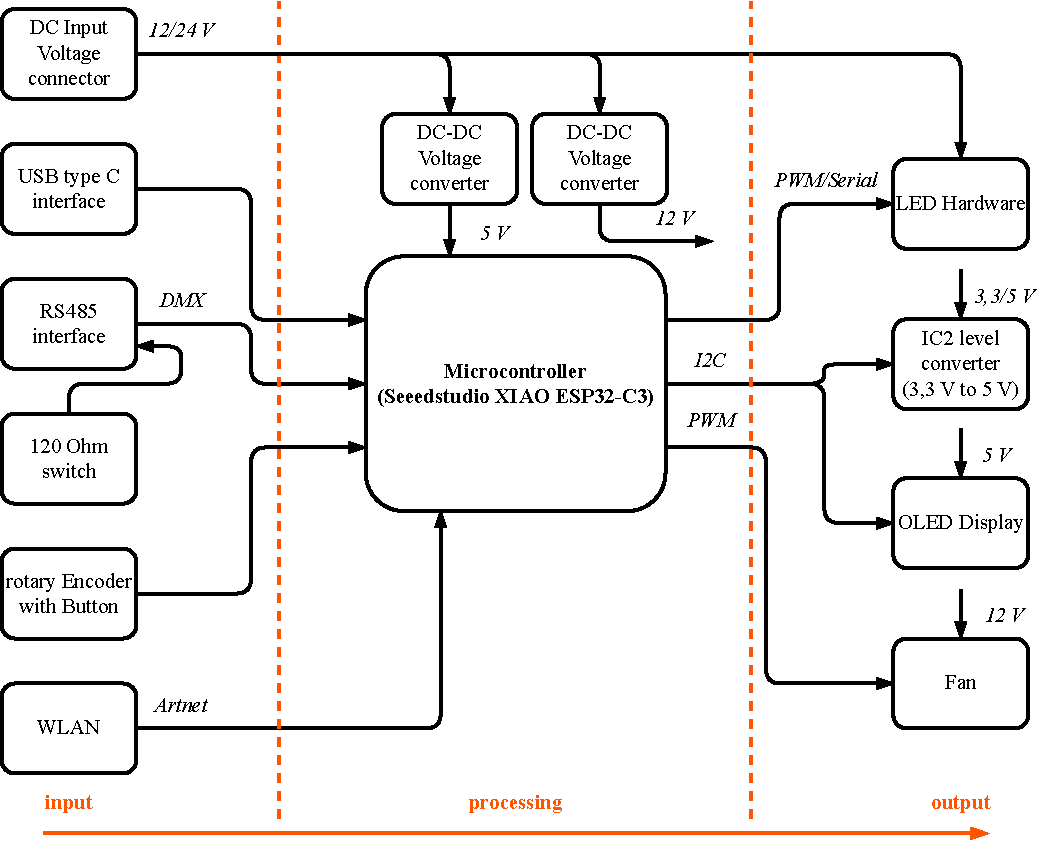
\includegraphics[width=0.95\linewidth]{graphics/hardware_architecture}
	\caption{Hardware System Architecture}
	\label{fig:hardwarearchitecture}
\end{figure}
The hardware architecture of the developed embedded \ac{LED} controller is segmented into three primary functional blocks: input, processing, and output. This design facilitates modularity and clear separation of concerns within the system. The schematic representation of this architecture can be seen in the provided diagram.

\subsubsection*{Input Block}

The input block is responsible for receiving power, data, and user commands.

\begin{itemize}
	\item \textbf{Power Supply:} The system accepts a flexible \ac{DC} input voltage ranging from 12V to 24V via a dedicated connector. This allows for compatibility with common power supplies found in lighting applications.
	\item \textbf{Programming and Debugging:} A \ac{USB} Type C interface is incorporated for firmware flashing, debugging, and potential serial communication during development.
	\item \textbf{Wired Communication:} An \ac{RS485} interface enables robust, long-distance wired communication, commonly used for protocols like \ac{DMX} in lighting control. A notable feature is an integrated switch to engage or disengage a 120 Ohm termination resistor, crucial for maintaining signal integrity in \ac{RS485} networks.
	\item \textbf{User Interface:} Direct user interaction is managed by a rotary encoder equipped with a push-button function. This allows users to navigate menus displayed on the \ac{HMI} and confirm selections.
	\item \textbf{Wireless Communication:} The controller integrates a 2.4 GHz \ac{WLAN} interface, enabling it to connect to standard wireless networks. This facilitates wireless control primarily through the Artnet protocol, a common standard for transmitting \ac{DMX} data over Ethernet networks.
\end{itemize}

\subsubsection*{Processing Block}

The processing block handles power regulation and executes the core logic of the controller.

\begin{itemize}
	\item \textbf{Power Conversion:} An essential component is the 5V DC-DC converter. This module steps down the incoming 12/24V supply to a regulated 5V. This stable 5V rail powers the sensitive electronic components, including the microcontroller and the display. \\
	For the spotlight a DC-DC converter provides a 12 V power rail. In this case, the input voltage does not match the fan voltage and is therefore needed. 
	\item \textbf{\ac{MCU}:} The central processing unit is the Seeedstudio XIAO ESP32-C3 microcontroller. This \ac{MCU} was chosen for its integrated Wi-Fi capabilities, sufficient processing power for handling communication protocols and control algorithms, and its compact form factor. It executes the firmware that manages inputs, processes control data (e.g., Artnet, \ac{DMX}), and drives the outputs.
\end{itemize}

\subsubsection*{Output Block}

The output block interfaces with the external components that the controller manages.

\begin{itemize}
	\item \textbf{\ac{LED} Control:} The primary function is controlling \ac{LED} hardware. The system is designed to support two main methods: direct serial communication for addressable \ac{LED} strips and \ac{PWM} control for driving different color channels (e.g., \ac{RGB}) of non-addressable \ac{LED}s.
	\item \textbf{Display Interface:} An \ac{I2C} interface is utilized to communicate with the \ac{OLED} display, which serves as the \ac{HMI}. In certain product configurations, such as integrated panel lights, this \ac{I2C} bus may also be used to send control data to other integrated components. An \ac{I2C} level converter is included to shift voltage levels between the 3.3V logic of the \ac{MCU} and the 5V requirement of the other peripherals. The display works with either 3.3V logic or 5V. To only drive the display, the level converter is not needed.
	\item \textbf{Thermal Management:} To ensure reliable operation, the controller incorporates fan control via a standard \ac{PWM} interface, compatible with typical computer fans. This allows the system to regulate its temperature under load.
\end{itemize}

\subsection{Hardware Configuration Options}
While the core architecture remains consistent, different hardware configurations and \ac{PCB}s are available to suit various application requirements:

\begin{itemize}
	\item \textbf{Tube Light V2 (Non-Addressable \ac{LED}s):} This variant utilizes hardware supporting three \ac{PWM} outputs for controlling non-addressable \ac{LED} strips. It omits the fan control output as it's not typically required for this configuration.
	\item \textbf{Tube Light V3 (Addressable \ac{LED}s):} For tube lights using addressable \ac{LED}s, the hardware provides support for a serial data output. Similar to the non-addressable version, fan control is not included.
	\item \textbf{Panel Light:} This configuration uses the same fundamental hardware as the addressable \ac{LED} tube light (serial output capable). However, the \ac{RGB} data for the panel is specifically transmitted via the \ac{I2C} interface instead of the dedicated serial \ac{LED} output. This version includes the hardware connection for fan control.
	\item \textbf{Spot Light:} The spot light employs an individual \ac{PCB} design tailored to its needs. It features three \ac{PWM} outputs for \ac{LED} control and includes the hardware connection for fan control.
	The size of the \ac{PCB} is designed to fit within the casing. The previous \ac{PCB} would not fit.
\end{itemize}

These variations ensure that each product type has an optimized hardware platform based on the core controller design, omitting unnecessary components or adapting interfaces as needed for the specific application.

\subsection{Software Architecture for Multi-Configuration Support}
\subsubsection{Interfaces between software modules}
The software is structured around a central main.cpp file as seen in figure \ref{fig:softwareinterfaces}. 
Interactions between various hardware abstractions and logic modules are orchestrated there.
\begin{figure}[H]
	\centering
	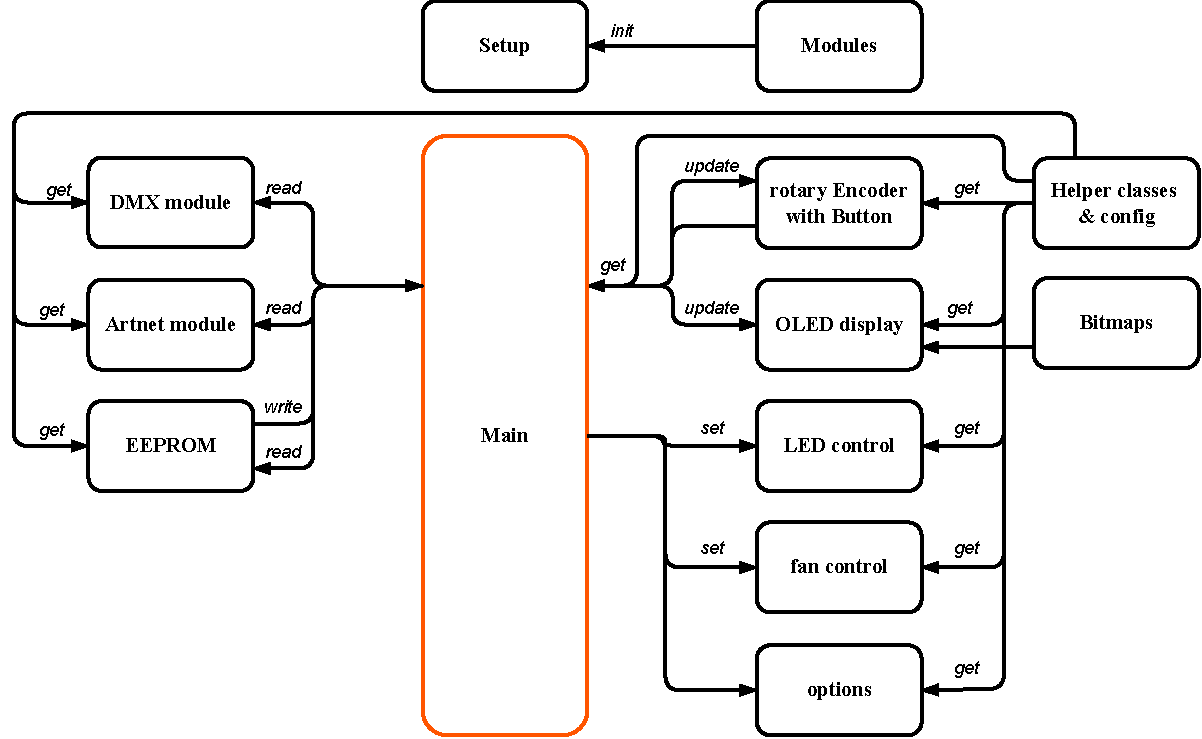
\includegraphics[width=0.95\linewidth]{graphics/software_interfaces}
	\caption{Interfaces of the software modules}
	\label{fig:softwareinterfaces}
\end{figure}
The software architecture features a central \texttt{Main} module (\texttt{main.cpp}) that coordinates interactions between several specialized modules. During startup, \texttt{Setup} initializes all other modules, including those managing hardware inputs (like the \texttt{Rotary Encoder}), outputs (\texttt{OLED Display}, \texttt{LED Control}, \texttt{Fan Control}), communication (\texttt{DMX Module}, \texttt{Artnet Module}), and data persistence (\ac{EEPROM}). \\

In the main loop, the \texttt{Main} module continuously polls the \texttt{Rotary Encoder} for user input events using getter functions. Based on the application state and user input, \texttt{Main} sends commands to update the \texttt{OLED Display} and control the \ac{LED} outputs via their respective modules. If enabled, fan speed adjustments are communicated to the \texttt{Fan Control} module.\\

Communication data for \ac{DMX} and Artnet is handled through dedicated modules. \texttt{Main} periodically checks for incoming \ac{DMX} data and initiates Artnet data parsing, receiving Artnet packets via a callback mechanism. Configuration and status information are exchanged using getter and setter methods provided by these communication modules.\\

Persistent storage of configuration settings is managed by the \ac{EEPROM} module, which provides interfaces for reading and writing the state of core application objects upon request from \texttt{Main}. Shared configuration values and helper classes containing state information are accessed by various modules as needed, typically through getter and setter methods.\\

\subsubsection{Main Loop}
The firmware executed by the \ac{MCU} operates based on a main execution loop, which continuously performs a sequence of tasks to manage the controller's functions. This loop is structured to ensure timely polling of inputs, processing of user interactions, and handling of communication protocols. \\

Initially, the loop polls the current state of all relevant hardware modules and software components, gathering the latest information. Following the polling stage, user input from the rotary encoder's push button is processed; the software distinguishes between short and long presses to enable different actions or menu navigation commands. Subsequently, changes in the rotary encoder's value are handled, typically translating these changes into menu navigation or parameter adjustments within the \ac{HMI}. \\

The loop then manages the state of the \ac{OLED} display, including standby or sleep modes, and updates the fan speed via \ac{PWM} based on thermal requirements or configuration (where applicable). Finally, several tasks are handled periodically within the loop's cycle. These include checking for the arrival of new \ac{DMX} data via the \ac{RS485} interface, managing the \ac{WLAN} connection for Artnet communication, and processing any received Artnet data packets. This structured, sequential, yet periodically interrupted approach ensures that all essential functions, from direct user interaction to network communication and output control, are managed efficiently within the controller's processing cycle.

\subsubsection{Menu Structure}
User interaction with the device primarily occurs through the rotary encoder and its integrated push button, as depicted in the menu structure diagram figure \ref{fig:menustructure}.
\begin{figure}[H]
	\centering
	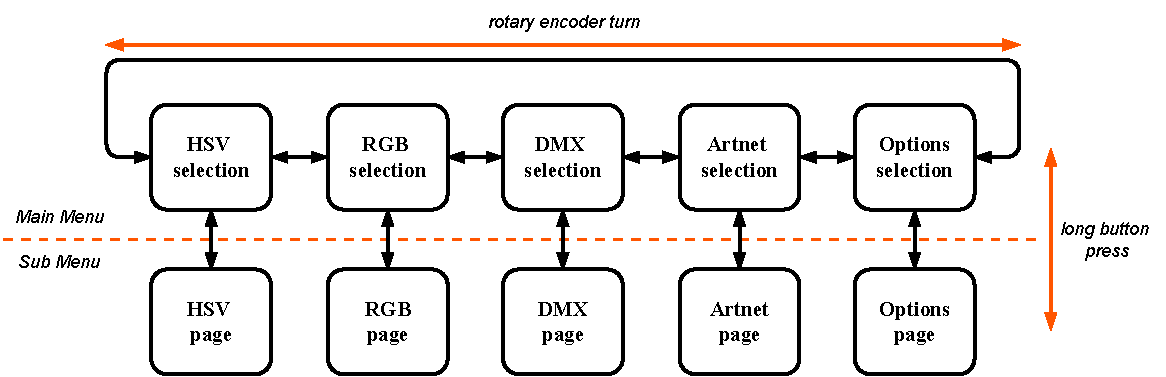
\includegraphics[width=0.95\linewidth]{graphics/menu_structure}
	\caption{Structure of the main menu navigation}
	\label{fig:menustructure}
\end{figure}

In the main menu view, turning the rotary encoder allows the user to cycle horizontally through the available function selections (such as \acs{HSV}, \ac{RGB}, \ac{DMX}, Artnet, and Options). The diagram confirms that this selection behavior includes wrap-around; if the user continues turning the encoder after reaching the first or last menu item, the selection jumps to the opposite end of the menu list, enabling continuous scrolling.\\

Vertical navigation between the main menu level and the corresponding submenu pages is achieved via a long press on the encoder's button. Performing a long press while a main menu item is selected transitions the software into that item's specific submenu, displaying its parameters or options. Conversely, performing another long press while within a submenu returns the user to the main menu selection screen. This hierarchical navigation, visually represented in the provided diagram, allows access to different functionalities and their settings using simple rotary and press actions.
	\newpage
	\section{Hardware Development}
\label{sec:hardware_development}

\subsection{Common Hardware Packages}
\subsection{Hardware Variations for Light Tube}
\subsection{Hardware Variations for Panel}
\subsection{Hardware Variations for Spotlight}
\subsection{Schematic Design}
\subsection{PCB Design and Fabrication}
\subsection{Component Selection and Justification}
\subsection{Component Assembly}
	\newpage
	\section{Mechanical Design and Enclosure}
\label{sec:mechanical_design}

\subsection{Light Tube Enclosure V2}
\label{subsec:light_tube_enclosure_v2}
\begin{itemize}
	\item Describe the design of the Light Tube enclosure using aluminum profiles and 3D printed end caps or mounting elements.
	\item Discuss the selection of aluminum profiles (e.g., size, shape).
	\item Detail the design and manufacturing process of the 3D printed parts.
	\item Mention any design considerations (e.g., light diffusion, mounting options, cable management).
\end{itemize}

\subsection{Light Tube Enclosure V3}
\label{subsec:light_tube_enclosure_v3}
\begin{itemize}
	\item Describe the design of the Light Tube enclosure using aluminum profiles and 3D printed end caps or mounting elements.
	\item Discuss the selection of aluminum profiles (e.g., size, shape).
	\item Detail the design and manufacturing process of the 3D printed parts.
	\item Mention any design considerations (e.g., light diffusion, mounting options, cable management).
\end{itemize}

\subsection{Panel Enclosure}
\label{subsec:panel_enclosure}
\begin{itemize}
	\item Describe the design of the Panel enclosure, primarily using 3D printed parts.
	\item Detail the design and manufacturing process of the 3D printed enclosure components.
	\item Mention any design considerations (e.g., rigidity, mounting options, heat dissipation).
\end{itemize}

\subsection{Spotlight Enclosure}
\label{subsec:spotlight_enclosure}
\begin{itemize}
	\item Describe the design of the Spotlight enclosure, primarily using 3D printed parts, including the 60° focusing mechanism.
	\item Detail the design and manufacturing process of the 3D printed enclosure components and the focusing element.
	\item Mention any design considerations (e.g., light focusing accuracy, heat dissipation, mounting options).
\end{itemize}

\subsection{Connection System \enquote{click \& hope}}

\subsection{Connection System \enquote{screw it!}}

\subsection{3D Printing}

\subsubsection{Light Tube V2 Parts}

\subsubsection{Light Tube V3 Parts}

\subsubsection{Panel Parts}

\subsubsection{Spotlight Parts}

\subsubsection{Connection System Parts}

\subsection{Threaded inserts}
	\newpage
	\section{Device Assembly} \label{sec:device_assebly}

	\newpage
	\section{Software Development}
\label{sec:software_development}
\subsection{Development Environment and Tools}
\subsection{Hardware Configuration Management in Software}
\subsection{LED Control Implementation for Different Products}
\subsection{Core Functionality Implementation}
\subsection{Communication Protocol Implementation}
\subsection{User Interface Implementation}
\subsection{Library Version Management}

	\newpage
	\section{Results}
\label{sec:results}
\subsection{Hardware Performance}
\subsection{Software Performance}
\subsection{Overall System Functionality for Each Product}
\subsubsection{Light Tube V2 (PWM Control)}
\subsubsection{Light Tube V3 (RGB IC Control)}
\subsubsection{Panel Light}
\subsubsection{Spot Light}
\subsection{Enclosure Quality and Durability}
\label{subsec:enclosure_quality}
\begin{itemize}
	\item Present observations and any testing results related to the quality and durability of the 3D printed and aluminum enclosures.
\end{itemize}
	\newpage
	\section{Conclusion}
\label{sec:conclusion}
\subsection{Summary of Work}
\subsection{Future Work}
\begin{itemize}
	\item Could include potential improvements to the enclosure designs or manufacturing processes.
\end{itemize}
	\newpage
	\section{Appendices}
\label{sec:appendices}

\subsection{Schematic Diagrams}
\subsection{PCB Layout}
\subsection{Source Code}
\subsection{Bill of Materials (BOM)}
\subsection{Datasheets}

\subsection{CAD Models and Drawings of Enclosures}
\label{subsec:cad_models}
\begin{itemize}
	\item Include CAD models or technical drawings of the 3D printed parts and the aluminum profile assemblies for each product variation.
\end{itemize}
	\newpage
	
	%\section{Problemstellung}\label{Kap:problemstellung}
\subsection{Aktueller Stand}


	%\newpage
	
	%%%%%%%%%%%%%%%%%%%%%%%%%%%%%%%%%%%%%%%%%%%%%%%
	%%%%%%%%%%  Literature and Appendix
	%%%%%%%%%%%%%%%%%%%%%%%%%%%%%%%%%%%%%%%%%%%%%%%
	\fancyhf{} % Clear all header and footer fields
	% switch page numberin to roman
	\pagenumbering{Roman}

	% set counter for page numbering.
	% !!!!!!!!!!!!!!!!!!!!!!!!!!!!!!!!!!!!!!!!!!!!!!
	% !!!!!!!!!!!!!!!!!!!!!!!!!!!!!!!!!!!!!!!!!!!!!!
	% Has to be done manually !!!!!!!!!!!!!!!!!!!!!!
	\setcounter{page}{7}

	% Literature
	\phantomsection
	\addcontentsline{toc}{section}{References}
	\bibliography{./includes/literatur}
	\newpage

	% Appendix
	%\appendix

	% Pack den Anhang hier rein
	%\include{./chapter/Anhang}

\end{document}